\documentclass[a4paper,oneside,article,11pt]{memoir}

\usepackage[english]{babel}
\usepackage[utf8]{inputenc}
\usepackage{amsmath,amssymb,amsthm}

\newtheorem*{toprove}{At bevise}
\newtheorem{mydef}{Definition}

% This font looks so good.
\usepackage[sc]{mathpazo}
\usepackage{fancybox}
% Typesetting pseudo-code
\usepackage{algorithm}
\usepackage{algorithmic}
\usepackage{multirow}
% Code comments like [CLRS]
\renewcommand{\algorithmiccomment}[1]{\makebox[5cm][l]{$\triangleright$ \textit{#1}}}
\usepackage{framed,graphicx,xcolor}
\usepackage{listings}
\usepackage{hyperref}

\usepackage[font={small,it}]{caption}

% Relative references
\usepackage{varioref}

\usepackage{tikz}

\bibliographystyle{plain}

\title{Bioinformatics - Tree Comparison \\ Project 1}
\author{Peter Gabrielsen 20114179\\
Christoffer Hansen 20114637}
\newcounter{qcounter}

\makeatletter
\newenvironment{CenteredBox}{% 
\begin{Sbox}}{% Save the content in a box
\end{Sbox}\centerline{\parbox{\wd\@Sbox}{\TheSbox}}}% And output it centered
\makeatother

\begin{document}

\maketitle

\chapter*{Introduction}
%A short status of your work. Does everything work as expected, or are there any problems or unsolved issues.
This project deals with implementing Day's algorithm for computing the RF distance between two unrooted trees over the same set of species. We present experiments where we compare the evolutionary trees constructed using the Neigbor Joining (NJ) methods implemented as \texttt{QuickTree} and \texttt{RapidNJ} on different datasets which were computed using align methods \texttt{Clustal Omega}, \texttt{Kalign}, \texttt{MAFFT} and \texttt{MUSCLE}.\\ \\Everything works as expected.
\\\\Code can be found at \url{https://dl.dropboxusercontent.com/u/8990890/2015Q2_AiBST_20114179_20114637_Project1.zip}.

\pagebreak

\chapter*{Implementation}

We implemented \texttt{rfdist} using Day's algorithm as presented in class. The only place we deviate from the algorithm is on sorting the collected intervals. We decided to do this using \texttt{QuickSort} instead of \texttt{RadixSort}. We are aware that this design choice makes an expected $\mathcal{O}(n \log n)$ algorithm, but as \texttt{QuickSort} is shown to perform well in practice, we did not consider this as being a problem.

The implementations is done in \texttt{c++}. It compiles using \textit{make rfdist} and runs using \textit{./rfdist $<$tree1$>$ $<$tree2$>$}, where \textit{$<$tree1$>$} and \textit{$<$tree2$>$} should be valid paths to files containing trees in well-formed \texttt{Newick}-format.

Correctness was tested on the provided \textit{testdata.zip} example.

\chapter*{Experiment 1}
\textit{For each alignment method ClustalW2 (1), Kalign (2), MAFFT (3), MUSCLE (4), we build a NJ tree using QuickTree and RapidNJ, and compute the RF-distance between each combination of these eight tree. The outcome of our experiment, an 8x8 table showing the RF-distance between each pair of constructed trees, is presented in figure~\ref{lst:experiment1}.} \\
\begin{figure}[H]
\begin{CenteredBox}
\begin{lstlisting}[]
	(1)NJ (2)NJ	(3)NJ	(4)NJ	(1)QT	(2)QT	(3)QT	(4)QT
(1)NJ	0	222	192	242	230	258	256	284	
(2)NJ	222	0	164	212	228	198	222	268	
(3)NJ	192	164	0	210	194	226	200	254	
(4)NJ	242	212	210	0	246	248	260	192	
(1)QT	230	228	194	246	0	158	114	198	
(2)QT	258	198	226	248	158	0	128	176	
(3)QT	256	222	200	260	114	128	0	182	
(4)QT	284	268	254	192	198	176	182	0
\end{lstlisting}
\end{CenteredBox}
\caption{Results of experiment 1}
\label{lst:experiment1}
\end{figure}

We are pleased to see the table is symmetric, as this is what we would expect.

\chapter*{Experiment 2}
\textit{The first experiment is done on the 395 input sequences in patbase\_aibtas\_permuted.fasta. This yields another 8x8 table presented in figure figure~\ref{lst:experiment2}.}

\begin{figure}[H]
\begin{CenteredBox}
\begin{lstlisting}[]
	(1)NJ (2)NJ	(3)NJ	(4)NJ	(1)QT	(2)QT	(3)QT	(4)QT
(1)NJ	0	210	172	246	238	264	252	280	
(2)NJ	210	0	176	252	250	230	246	276	
(3)NJ	172	176	0	238	268	268	244	286	
(4)NJ	246	252	238	0	216	242	232	208	
(1)QT238	250	268	216	0	138	108	158	
(2)QT264	230	268	242	138	0	124	172	
(3)QT252	246	244	232	108	124	0	148	
(4)QT280	276	286	208	158	172	148	0	
\end{lstlisting}
\end{CenteredBox}
\caption{Results of experiment 2}
\label{lst:experiment2}
\end{figure}

Again, we are are pleased to see the table is symmetric. This gives us confidence that our implementation is correct.

\chapter*{Experiment 3}
\textit{Compute the RF-distance between the trees produced in 'Experiment 1' and 'Experiment 2' using the same alignment and tree reconstruction method. This yields 8 distances presented in figure~\ref{lst:experiment3}.}

\begin{figure}[H]
\begin{CenteredBox}
\begin{lstlisting}[]
(1)NJ (2)NJ	(3)NJ	(4)NJ	(1)QT	(2)QT	(3)QT	(4)QT
160	200	184	216	68	62	42	158	
\end{lstlisting}
\end{CenteredBox}
\caption{Results of experiment 3}
\label{lst:experiment3}
\end{figure}


We conclude that aligning using \texttt{Clustal Omega} seems to perform the best on \texttt{RapidNJ} and that \texttt{MAFFT} seems to perform the best on \texttt{QuickTree} on the test data we have been experimenting on.

\chapter*{Experiment 5}

We test running time by computing perfectly balanced binary \texttt{Newick}-trees with height in the interval $k \in [2, \cdots, 23]$ giving a total number of nodes equal to $2^{k+1}-1$. As we double the number of nodes on each test-run we expect to see a straight line in a log-log plot. We are pleased that this is indeed the case, as presented in figure~\ref{fig:plot_running_time}.

\begin{figure}[h]
\centering
  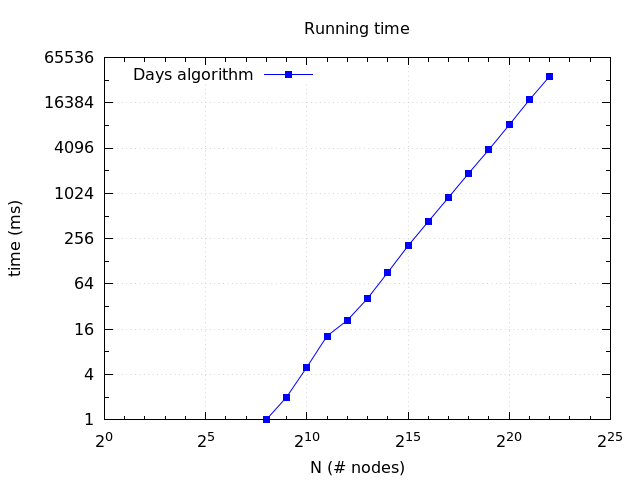
\includegraphics[width=\linewidth]{../running_time.png}%
  \caption{Running time of rfdist}
  \label{fig:plot_running_time}
\end{figure}


\bibliography{references}

\end{document}


